%!TEX root = ../master.tex
\chapter{Abbildungen}
Man kann viele verschiedene Dateiformate in LaTeX einbinden, die beste Variante sind jedoch Vektorgrafiken. Diese sind beliebig skalierbar und sind somit immer gut zu lesen bzw. nie verpixelt. Wenn man Pixel-Grafiken verwendet sollte immer darauf geachtet werden, dass eine möglichst hohe Auflösung der Datei sichergestellt wird. 
 \begin{figure}[H]
    \centering
    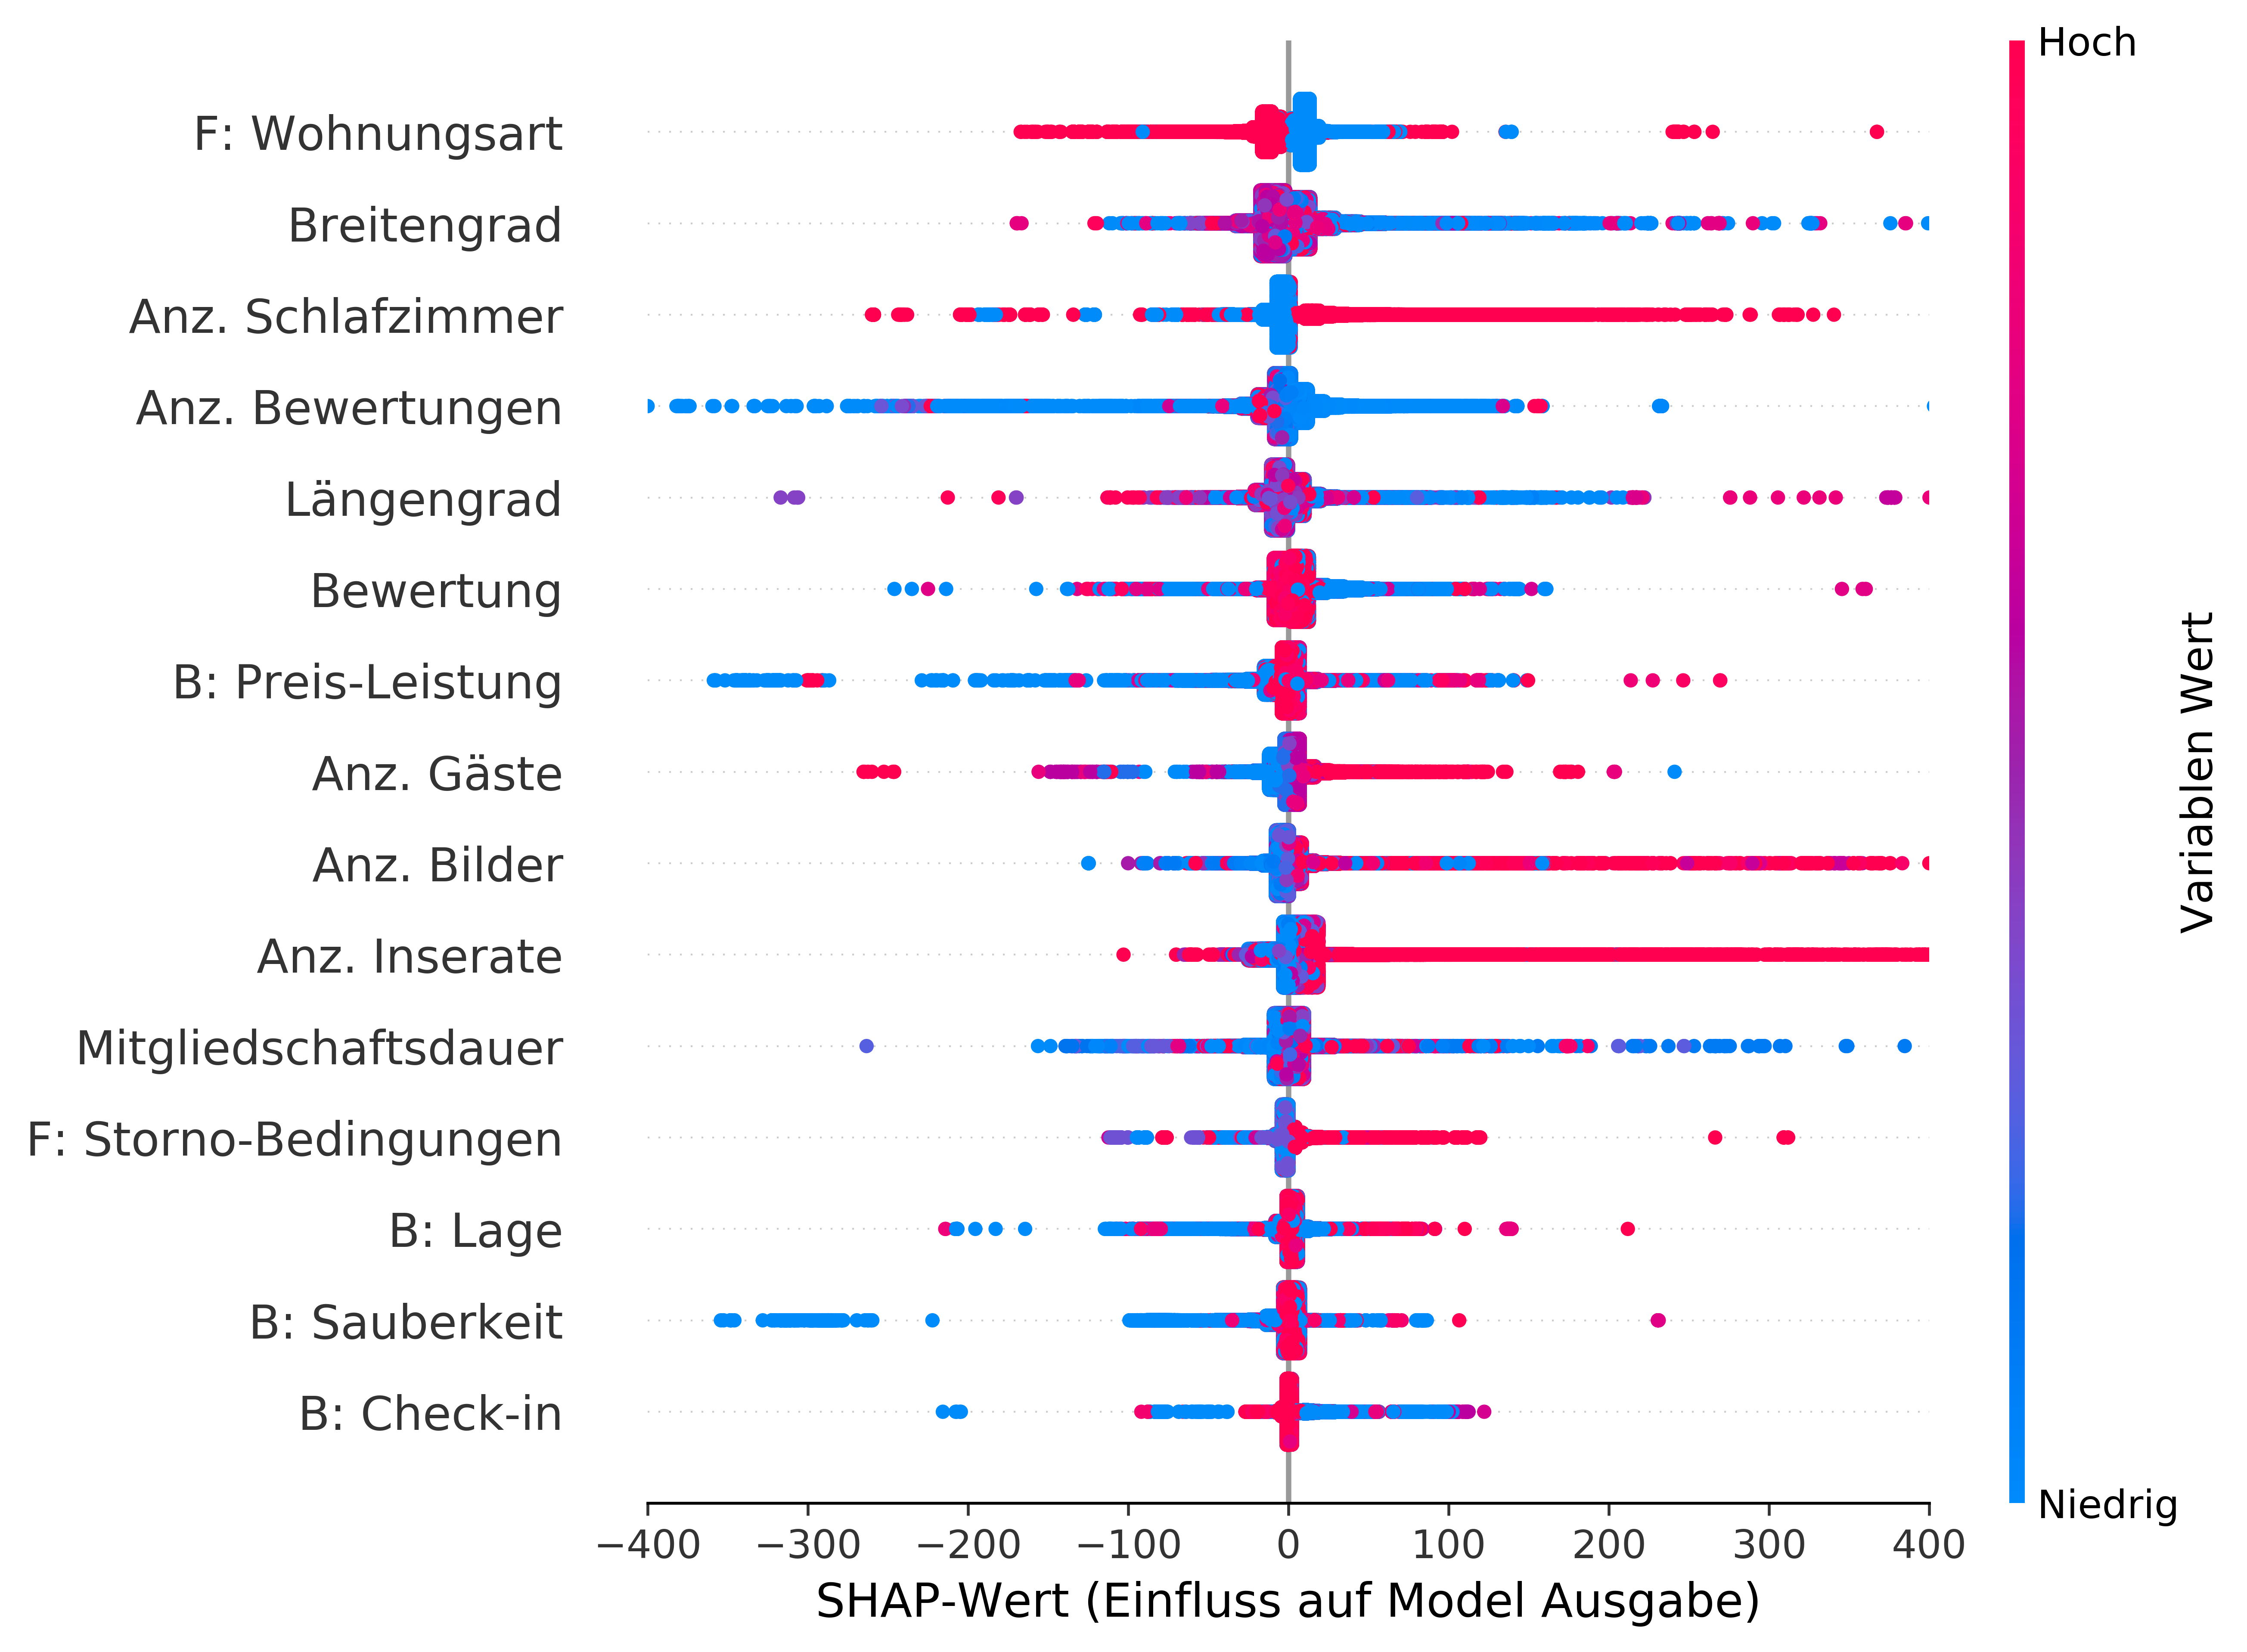
\includegraphics[width=0.8\linewidth]{graphics/summary.png}
    \caption{Abbildung der SHAP-Werte für die 15 wichtigsten Variablen}
    \label{fig:SHAP}
\end{figure}  
Um Bilder in LaTeX einzubinden wird die Umgebung \emph{figure} verwendet. In dieser wird über den Befehl \emph{\textbackslash includegraphics[Optionen]\{Dateipfad\}} die Datei aufgerufen. Eine besonders interessante Option ist \emph{width=0.8\textbackslash linewidth} welche dafür sorgt, dass die Abbildung immer genau gleich groß ist, nämlich genau 80\% der Textweite. \\
Auch auf Abbildungen kann verwiesen werden (Abbildung \ref{fig:SHAP}).